\documentclass[12pt]{article}
\usepackage[numbers]{natbib}
\usepackage[margin=1in]{geometry}
\usepackage[nottoc]{tocbibind}
\usepackage{setspace}
\usepackage{svg}

\graphicspath{{../out/graphs/}}

\doublespacing

\author{Thomas Kwashnak}
\title{Comparing Performance of Machine Learning Libraries with Manual Implementations}

\newcommand{\CC}{C\nolinebreak\hspace{-.05em}\raisebox{.4ex}{\tiny\bf +}\nolinebreak\hspace{-.10em}\raisebox{.4ex}{\tiny\bf + }}

\begin{document}

\maketitle

\newpage

\section{Abstract}

Machine learning often uses simple-to-use languages and libraries such as Python and TensorFlow.
While learning and using these frameworks may be easier, there is the possibility that some overhead cost is assumed.
While seemingly small, if a model using these frameworks is brought into production, the time lost can easily build up to an actual cost increase for running.
This paper seeks to understand the difference, if any, between using these frameworks and manually implementing the algorithm in bare-bones code.
Implenetations of a neural network back propagation algorithm is implemented in Rust, Python with TensorFlow, and CUDA/\CC, and the run-time is compared on identical datasets.
The results indicate that the raw CUDA performed thousands of times better than the TensorFlow, which performed significantly better than the manual Rust implementation.
Thus, the conclusion is drawn that in performance-critical applications, spending time manually implementing the model has the potential to have long-term cost savings.
However, it should not be disregarded the ability for rapid prototyping and quick implementation that TensorFlow and Python provides.


\section{Introduction}

% \paragraph{Intro Paragraph}
\paragraph{}
Machine learning is a quickly-growing industry with the recent boom of generative AI.
Many companies and organizations are quickly trying to use these machine learning frameworks for their own purposes.
However, these models are expensive, and can quickly spike up server cost to run.
These machine learning implementations are often using libraries such as TensorFlow \cite{lib_tensorflow} and PyTorch \cite{lib_pytorch} are often considered the standard for performing more complicated machine learning tasks.
These libraries handle a significant amount of the underlying methods used, and provide the ability to even utilize a GPU if it has the correct framework.
However, these libraries are mainly interacted with through the Python language \cite{lang_python}, which is often noted to be a slow language.

% \paragraph{Review of Python as a growing language / use in Data Science}
\paragraph{}
Python has been one of the fastest growing languages in the industry today \cite{article_python_growing_language}.
Srinath, in their paper discussing Python's growing popularity, discusses several factors that lead to Python's success.
The Python language is an interpreted and dynamically typed language.
This, along with the very simple syntax, makes Python very quick to learn and start using.
It's highly extensible, and many mature libraries and frameworks that make even some complex tasks trivially easy to implement in Python.
One of the industries that Python continues to excel at is the data science and engineering community, where libraries in Python simplify working with databases or datasets.
The only drawback to Python is that it sacrifices speed for the ability to be as flexible as it is.
This can be partially mitigated, as Python allows building Python libraries from \CC  or other languages.
However, this doesn't fully eradicate the drawbacks to a dynamically typed interpreted language.

% \paragraph{Review Compiled vs Interpreted Language}
\paragraph{}
There are three general types of translation modes for programming languages; interpreted, hybrid, and compiled \cite{article_compiled_interpreted_hybrid_languages}.
Python, and other similar languages, fall under the interpreted category.
Interpreted languages are typically taken line by line, executed immediately.
This allows for languages to be more portable as the interpreter interprets the inserted code, and runs machine level code based on the condition.
Hybrid languages include languages like Java.
The written code is first converted into byte-code, and then run on a virtual machine that can be platform dependant.
Compiled lanugages, such as C and \CC, compile code into machine-specific instructions that can be executed as is.
There are tradeoffs and benefits of using each these translation modes.
Interpreted and Hybrid languages are highly portable, as they rely on a virtual machine or the interpreter to convert code to device instructions.
However, they sacrifice execution time as additional checks and parsing happens when the program executes.
Compiled languages, however, are typically more strict with syntax, but they provide significantly better runtime performance than interpreted or hybrid languages.
That is to say, that code written in C and \CC are typcially faster to run than Python, but may be more difficult to impement or iterate on because of the language syntax and patterns.

% \paragraph{Review of Deep Learning Framework Debt}

\paragraph{}
Libraries are pre-built collections of code that make it easier for developers to implement and perform certain tasks.
Often times, libraries are generalized to be used in a multitude of situations.
Thus, it's also important that these libraries are as efficient as they can be.
A recent study took a particular look into popular deep learning libraries, such as TensorFlow and PyTorch, and inspected the comments that indicate technical debt existing in the code \cite{article_deep_learning_framework_debt}.
The researchers categorized these indications of technical debt into categories; design debt, defect debt, documentation debt, test debt, requirement debt, compatability debt, and algorithm debt.
They found that the majority of technical debt found fell under design debt, followed by requirement debt and algorithm debt.
This indicates that there are a lot of areas within popular deep learning frameworks that the developers wish they had more time to fix, polish up, or change.
The conclusion is that these widely used libraries aren't without defects and shortcomings.
Thus indicating that use of these frameworks may assume some overhead.


% \paragraph{Review of Neural Networks}

\paragraph{}
Neural networks is a category of mathematical models under machine learning that loosely attempts to mimick the brain \cite{book_intro_neural_networks}.
They are composed of nodes, or neurons, that accept multiple inputs from previous nodes, each value weighted by some unique weight, and outputs some value based on the inputs.
Neural networks have the ability to drastically increase its size, in turn increasing the time it may take to run the model on a given inputs.
The architecture of neural networks lends itself well to being represented using linear algebra, which itself lends nicely to parallelization and other optimizations.

% \paragraph{Summarize the problem statement
\paragraph{}
In the data science industry, many times models using TensorFlow or PyTorch are sent into production without additional optimization.
The question lies in how much performance impact, if any, does this entail.
That is, what is the balance between being able to develop quickly, or avoiding interpreted languages and large libraries to hopefully improve execution performance.
This paper seeks to explore the performance difference between manual implementations on both the GPU and CPU, compared to implementations using Python \cite{lang_python} and TensorFlow \cite{lib_tensorflow} when using either the GPU or CPU.

\section{Methods}

% \paragraph{Initial Discussion of Methods}

\paragraph{}
To test the performance difference between manual implementations and the TensorFlow library, an identical algorithm was implemented in multiple different frameworks and languages.
This includes CUDA \cite{lib_cuda}, which runs on the GPU, TensorFlow \cite{lib_tensorflow}, which runs on either the GPU or CPU, and Rust \cite{lang_rust}, which acts as the CPU implementation.
While identical algorithms were not feasable to implement during the alloted time frame, each algorithm attempts to be as fast is it can be for the particular framework.
The algorithm chosen is a simple back-propagation neural network.
This allows for experimenting with the number of variables and size of the network, as well as the number of observations being concurrently processed at once.


\paragraph{Neural Network}

The main algorithm implemented in this paper is neural network back propagation.
The neural network used in this paper is a dense neural network with 6 hidden layers, each with the same number of nodes as there are input variables.
The output layer only contains a singular node, which is what we will be testing against.

Back propagation is one of the main methods of training neural networks.
In back propagation, the neural network is fed a set of inputs.
It then compares the value it gets from the output node with the expected value of the output node.
The back propagation algorithm then propagates the error back through the neural network, calculating the error of each weight and bias.
The weights and biases are then updated to try and reduce the error for the provided inputs.
In this paper, several inputs are provided at once, and the weights and biases are nudged based on the average error of all observations.

While this process is not exactly the same in each of the implementation, it is done close enough to compare how fast each implementation is able to run the model.
Because we are focusing on execution time and not accuracy of the model, the implementations may not be exactly the same, but should roughly have the same runtime needed for each proper implementation.


\paragraph{Data Generation}
In order to maintain as much consistency between the implemented models, a central dataset and values are created and used by each of the implementations.
The dataset is completely randomly generated using Python \cite{lang_python}, and configured using a TOML file.

There are two scaling sliders in the data generating process; Number of variables and number of observations.
The number of variables handles how many inputs there are in the input of the neural network, as well as how large the hidden layers are.
The number of observations handles how many entries are sampled from the dataset during each iteration.

The data generation script outputs several artifacts used by the models.
First, it outputs a separate dataset for each number of variables.
It also outputs the size and initial weights and values of the neural network itself.
Then, it generates bootstrap samples from the original dataset.
Each bootstrap sample contains a list of indexes from the dataset to pull for that iteration.
To grab a bootstrapped sample of the specified number of observations, the first $n$ indexes from the bootstrap are gathered.

Each implementation of the neural network back propagation algorithm accepts environment variables that point the code to where it should grab the data from.
A Bash script is used to iterative run each model for each of the combinations of observation counts and variable counts.

\paragraph{Rust}

The Rust \cite{lang_rust} implementation acts as the CPU implementation within this paper.
Custom structs are made to handle each individual layer and the collection of layers together.
The weights and values are stored in 64-bit floats to provide as much precision as possible.
The feed-forward and back-propagation algorithms are implemented in the individual layers.
It should be noted that the back-propagation algorithm here does not change the values within the layer itself, but rather returns a new layer of nudges.
This allows for the model to be parallelized across observations, achieved by using the Rayon \cite{lib_rayon} crate.
After the observations are completed, the nudges are combined to obtain the ``average changes'' required for the model.
It is then properly scaled and applied to the neural network weights and values.


\paragraph{CUDA}

CUDA \cite{lib_cuda} is a specialized extension of \CC \cite{lang_c++} used to interact with supported NVIDIA GPUs.
The main beneift of using NVIDIA GPUs is the ability to create a Kernel, or set of code that runs fully parallel across several dimensions \cite{lib_cuda}.
This kind of optimization significantly shows its prowess with algorithms such as back-propagation.
In the CUDA implementation, the algorithm is parallelized across both the observations and number of variables being processed at that time.
This is done by splitting up the algorithm into multiple kernels.
First, feed forward is implemented as a kernel that pushes data from one layer to the next.
Then, a separate back propagation method is created to handle back propagating from the output node, since additional simplifications can be made.
For the rest of the layers, a more general back propagation kernel is used.
The back propagation process, similar to the Rust implementation, outputs several `nudge' vectors that contain the changes needed to make towards the weights and biases.
The final kernel handles applying those nudges to the weights and biases in the network.
In the implementation, 1-dimensional arrays are used to simplify the parameters, but they are still treated as if they were 2-dimensional arrays.
Finally, doubles are used for the weights to maintain the precision, similar to the Rust implementation.

\paragraph{TensorFlow}

The TensorFlow \cite{lib_tensorflow} implementation is implemented using a Python \cite{lang_python} script.
This implementation is remarkably different than the other two implementations given the particular way that TensorFlow accomplishes its tasks.
TensorFlow uses a graph-like model to optimize the calculation process, meaning that features such as back propagation doesn't need to be manually implemented.
In short, the implementation in Python runs the neural network's feed forward algorithm, calculates the loss based on the result, and uses gradient descent to update the weights and biases within the neural network.
While there are more encompassing implementations such as Keras, the goal of this implementation is an as-bare-bones implementation as possible of a back propagation neural network.

TensorFlow has the unique ability of running on both the GPU and CPU.
Thus, the TensorFlow implementation is able to be run twice, once on the GPU and again on the CPU.
By default, TensorFlow runs on the GPU, if any.
In order to negate this default behavior, the environment variable CUDA\_VISIBLE\_DEVICES is set to $-1$.
This forces TensorFlow to default back to the CPU-based implementation.

\paragraph{Running the Experiment}

The final experiment run in this model had the following configuration.
The number of observations initially generated is 1,000 observations.
Each dataset of observations ranged from 10 to 1,000 variables.
The implemented models were recorded in running 50 iterations, each time training on between 10 and 200 observations simultaneously.
The neural network consisted of 6 layers, each layer with an equal number of nodes to the number of variables in the data.

The experiment was run on a Windows 11 desktop using WSL.
The computer consisted of an AMD Ryzen 9 5900X CPU and a NVIDIA RTX 3080 GPU with 32GB of ram, and 10GB of VRAM on the GPU.
The code can be found in the GitHub Repository LittleTealeaf/CSC-Senior-Thesis\footnote{https://www.github.com/LittleTealeaf/CSC-Senior-Thesis}.

In tracking the average execution time for each implementation, data loading and unloading was not tracked.
That is, the variables and data is loaded into the GPU or RAM before the timer starts, and is unloaded after the timer ends.
This keeps the measured time closer to just focusing on the time taken to execute the entire process.

Once the data is collected, it is combined into a single CSV dataset using a simple Bash script.
It is then loaded into R \cite{lang_r} and graphed using the R libary ggplot2 \cite{lib_ggplot2}.

\section{Results}

\begin{figure}
	\begin{center}
		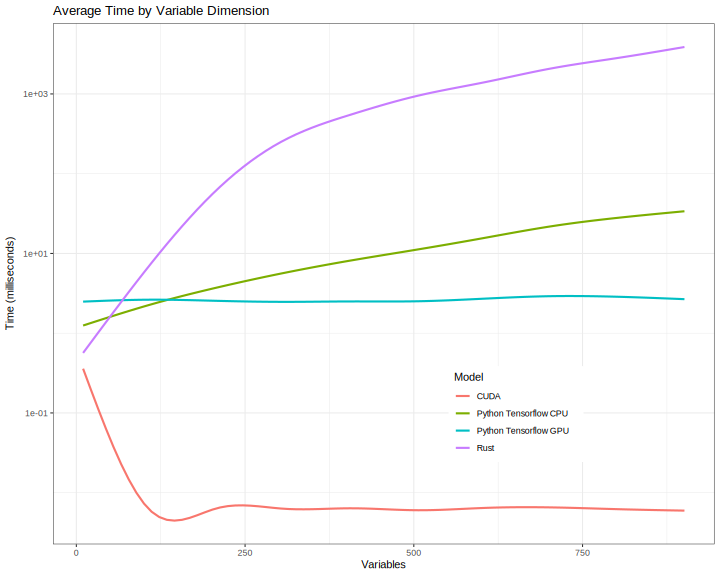
\includegraphics[width=0.9\linewidth]{variables.png}
	\end{center}
	\caption{Average time taken to run through one iteration of back propagation based on the number of variables. Time is on a $\log_{10}$ scale. Lines show trends in the data, using ggplot2 geom\_smooth \cite{lib_ggplot2}.}
	\label{fig:graph:variables}
\end{figure}

\begin{figure}
	\begin{center}
		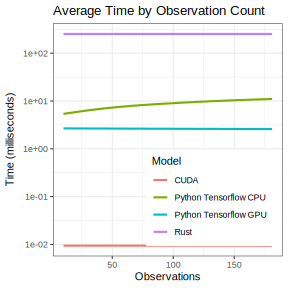
\includegraphics[width=0.9\linewidth]{bootstraps.png}
	\end{center}
	\caption{Average time taken to run through one iteration of back propagation based on the number of concurrent observations processed at a time. Time is on a $\log_{10}$ scale. Lines show trends in the data, using ggplot2 geom\_smooth \cite{lib_ggplot2}.}
	\label{fig:graph:observations}
\end{figure}

\paragraph{}
Figure \ref{fig:graph:variables} depicts the average time taken for each of the models based on the number of variables, and therefore the size of the network.
At very low variable counts, all the models had a relatively similar average runtime.
However, as the number of variables increases, the models seem to diverge significantly.
Rust, the slowest at high variable count, increases exponentially as more variables are added.
In higher variable counts, it increased to an average of over 1 second per iteration.
The TensorFlow on the CPU was the second slowest implementation.
Similar to Rust, the average runtime exponentially increases as varaibles are added.
However, the rate that the Tensorflow CPU runtime increases is significantly slower than Rust, so while it starts out slower than Rust, it quickly becomes nearly hundreds of times faster than Rust.
Tensorflow on the GPU makes almost no visible change in runtime.
It consistently maintains around 5 ms average execution time.
However, it proves to be significantly slower compared to CUDA, which presented interesting behavior.
In very low variable counts, CUDA had a slower runtime more in line with the other implementations.
However, it quickly drops down and plateaus to significantly lower than any of the other implementations.
In higher iterations, the CUDA implementation performed 1,000x or so bette than TensorFlow on the GPU, the second fastest implementations.

\paragraph{}
Figure \ref{fig:graph:observations} show the average time taken for each of the models based on the number of observations concurrently trained on for each of the iterations.
Each of the implementations had very little difference in runtime when the number of observations changed.
The only implementation that showed any noticeable difference was the TensorFlow implementation when running on the CPU, where the runtime slowly increased as more observations were added.
However, the increase is significantly lower than those shown in Figure \ref{fig:graph:variables}.

\section{Discussion}

\paragraph{}
To start off with the least significant results. In Figure \ref{fig:graph:observations}, it shows that only the TensorFlow on CPU implementation had any change at all when the number of concurrent observations increased, and even then it is not too significant.
This makes sense given the way that each handles parallelizing the executions.
Rust, for starters, specifically only parallelizes across observations using the Rayon \cite{lib_rayon} crate.
That is, it should be expected that adding more observations per iteration wouldn't have too much of a difference in the runtime.
CUDA, similarly, also parallelizes across observations.
Thus, CUDA also doesn't significantly change its runtime when adding additional variables. 
The same can be said with the GPU implementation of TensorFlow, since the GPU parallelizes across observations naturally.
However, the same cannot be definitely said in the CPU implementation of TensorFlow.
The detailing of the implementation of TensorFlow was not within the context of this paper, so it cannot be stated whether or not it parallelizes on the CPU.
However, it should be noted that it still performed faster than Rust, indicating that there are several methods of optimizations that have been used to push its performancce as far as it can.

\paragraph{} % CPU increase exponentially, GPU don't increase as much. Discuss how the variable count significantly impacts the size of the network, and how the parallelization acorss variables is important
One of the significant differences between the CPU implementations and GPU implementations is the effects of larger number of variables, and by extension size of the neural network.
This type of effect wasn't as noticeable in Figure \ref{fig:graph:observations} because the number of observations only has an effect on the number of concurrent observations fed into the network at the same time, while the number of variables affects every layer in the network's size.
In Figure \ref{fig:graph:variables}, it's very noticeable the difference between CUDA and TensorFlow GPU, and TensorFlow CPU and Rust.
Since the two GPU implementations handle parallelization of the variables in addition to the parallelization of observations, they are able to take more variables before slowing down even more.
However, since the CPU doesn't have the same ability of parallelization that the GPU has, we notice an exponential relationship between the number of variables and the average runtime of the algorithm.
While it might be possible to parallelize over variables on the CPU as it does in the GPU, it may have significant drawbacks, since the CPU has significantly less multithreading ability than the GPU.
As far as hardware is concerned, it can be concluded that the use of GPU to parallelize as much as possible provides significant improvements in performance.

\paragraph{} % Rust vs CPU Tensorflow
While both of the CPU implementations, Rust and Tensorflow CPU, had exponential relationships between variable count and average runtime, the TensorFlow implementation had a significantly slower increase.
Albeit the implementation of Rust was very basic and bare-bones, it still was fully compiled and fighting against a model implemented in an interpreted language.
At some points, the TensorFlow implementation on the CPU performed up to 100x faster than the Rust implementation.
While exploring the underlying technology behind TensorFlow's CPU implementation was out of scope for this paper, there are obviously several levels of optimization that TensorFlow has for CPU operations.
Is it possible for someone who is knowledgeable about these optimizations to out-perform TensorFlow? Definitely.
There is still the level of optimizations that can be gained simply by avoiding interpreted languages like Python \cite{article_compiled_interpreted_hybrid_languages}.
However, for a basic user looking to create and run models without too much deep-level knowledge, TensorFlow provides significant power to users working on a CPU.


\paragraph{} % CUDA vs TensorFlow GPU
The other pair of implementations to compare is the CUDA and TensorFlow on the GPU.
As shown in Figure \ref{fig:graph:variables}, there is a significant performance difference between the two implementations.
Across a wide range of variable counts, the CUDA implementation performed 1,000s times faster than the TensorFlow GPU implementation.
The only time where this wasn't the case was near the beginning, when there was a low variable count, and the runtime of CUDA was for some unknown reason closer to the other implementations.
However, it still doesn't change the significant lead that CUDA has against TensorFlow GPU.
There could be several reasons why this might be the case.
First, CUDA is a compiled language, and thus would naturally be faster than an interpreted language like Python running TensorFlow \cite{article_compiled_interpreted_hybrid_languages}.
Second, and more importantly, there might be a significant amount of overhead that TensorFlow includes.
TensorFlow takes a unique approach to their implementations. In order to make TensorFlow work on different infrastructures, and work for many different applications, an execution graph is generated to keep track of where values go.
When running, the execution graph first has to be generated, based on the operations made within the code.
Then, several optimization passes are run in order to attempt to improve the performance of the model.
However, these optimization passes can't be too specific or intense, as this is all running during execution.
Additionally, TensorFlow is a large library and has gone through several changes and accumulated a decent amount of technical debt \cite{article_deep_learning_framework_debt}.
Thus, there might be several possible optimization techniques that have not yet been implemented.
This makes TensorFlow even slightly slower than manual implementations.
On the contrary, when writing CUDA code the optimizations and execution plan need to be thought about and implemented beforehand.
This can be very complicated for developers that may not fully understand the strengths and weaknesses of working with CUDA.
However, once done the code can be run multiple times with significantly faster performance, as it does not need to handle optimizations or missing features during execution time.


\paragraph{} % Implementation Time
Execution time isn't the only factor in deciding what tools to use in a project.
While yes, manually implementing the algorithm in CUDA may out-perform TensorFlow, it requires a significant amount of knowledge.
During this project, implementing CUDA was one of the more difficult tasks.
Writing the Python code to implement both TensorFlow implementations took only a few hours, if not less.
However, CUDA took several days of planning out array indexing, grasping how CUDA managed data and parallelization, and bringing all the pieces together to a working algorithm
Even the Rust implementation took some time to get together, as it also required prior knowledge and experience with how back propagation works.
It should also be noted that implementing TensorFlow only needed to be written in Python once, and then it could be executed on either the GPU or CPU efficiently.
By creating an operation graph, the developers for TensorFlow are able to manually write separate code that uses the strengths and weaknesses of the architecture it runs on.

\section{Conclusion}

\paragraph{}
While manually implementing may provide significant performance improvements, the answer isn't so clear.
Manually implementing algorithms takes a deep level of knowledge of the algorithm itself, as well as the infrastructure that the algoritm is implemented on.
It also may take significantly longer to build, and may need to be scrapped any time there is a small change in the architecture of the model.
TensorFlow, however, paired with Python provides easy access to ``good-enough'' implementations that get the job done, and provides significant ease of development.
Small changes in the architecture can likely be handled by TensorFlow, with little changes needing to be made to the code itself.

\paragraph{}
Therefore, a balance has to be made between the two.
In situations where the model is rapidly changing and needs to be utilized as soon as possible, TensorFlow and other libraries provide amazing tooling and capabilities to make it happen.
However, in time-critical situations or more stable environments, especially those that allow the extra time needed to implement it, manually implementing the model has its beneifts too.
In some teams or companies, a combination might be found, where the development team builds the model using TensorFlow or other libraries, and then that is converted into a more low-level program by more experienced teams.

\paragraph{}
It should be noted that this project isn't fully encapsulating, and there is still work that can be done in the future.
First, it should be noted that the span of varaibles and observations recorded in this project are reduced in order to run within a reasonable time-frame.
Any larger spans would cause the experiment to take days or even weeks to run through every combination it needs to.
Additionally, the Rust implementation could gain significant improvements.
It should be feasable to build a Rust implementation that is comparable to or faster than the TensorFlow when run on the CPU.
Lastly, more research into the underlying technology of TensorFlow, as well as expanding this project to other libraries such as PyTorch, would expand the depth that conclusions can go as to the overhead of these libraries.

\paragraph{}
In conclusion, the answer isn't clear.
Python, in tandem with TensorFlow, provides the ability to rapidly prototype and easily implement complex algorithms with only a few lines.
CUDA, and other low-level languages, provide the ability to plan out and create programs that utilizes the strengths and weaknesses of the hardware to its fullest potential, without the overhead of generalized libraries.
Thus, it shouldn't be stated that using libraries are better than writing manually or vice versa, but rather that they are different approaches and each have their place in the field.



\newpage
\bibliographystyle{ieeetr}
\bibliography{refs}

\end{document}
